\documentclass[apjl]{emulateapj}

\include{vc}

\usepackage[english]{babel}
\usepackage[utf8x]{inputenc}
\usepackage{amsmath}
\usepackage{graphicx}
\usepackage[colorinlistoftodos]{todonotes}


\shortauthors{Barclay et al. 2013}
\shorttitle{Kepler-91\lowercase{b} is a giant low-density planet orbiting a giant low-density star}


\begin{document}
%\title{Radial velocity confirmation of a transiting 0.75 jupiter-mass planet orbiting the red giant star Kepler-91}
%\title{Confirmation of Kepler-91\lowercase{b} as a giant low-density planet orbiting a giant low-density star}
%\title{Kepler-91\lowercase{b} is a giant low-density planet orbiting a giant low-density star: an analysis utilizing radial velocity observations and Gaussian Process light curve noise modeling}
%\title{Radial velocity observations and light curve noise modeling reveal Kepler-91\lowercase{b} is a giant low-density planet orbiting a giant low-density star}
\title{Kepler-91\lowercase{b} is a giant low-density planet orbiting a giant low-density star}
% I kinda want to mention RV and GP in the title
\author{Thomas Barclay$^{1,2}$, Michael Endl$^{3}$, Daniel Huber$^{1,4}$,  Daniel Foreman-Mackey$^{5}$, William D. Cochran$^{3}$, Phillip J. MacQueen$^{3}$ and Elisa V. Quintana$^{1,4}$}

\slugcomment{To be submitted to a journal (ApJ? maybe MNRAS.)}

\altaffiltext{1}{NASA Ames Research Center, M/S 244-30, Moffett Field, CA 94035, USA}
\altaffiltext{2}{Bay Area Environmental Research Institute, 596 1st Street West, Sonoma, CA 95476, USA}
\altaffiltext{3}{McDonald Observatory, The University of Texas at Austin, Austin, TX 78712, USA}
\altaffiltext{4}{SETI Institute, 189 Bernardo Ave, Suite 100, Mountain View, CA 94043, USA}
\altaffiltext{5}{New York University, Center for Cosmology \& Particle Physics, New York, NY 10003, USA}


\begin{abstract}
Kepler-91b was detected using data from the Kepler spacecraft and its planetary nature was confirmed through analysis of the light curve. Recently these data have been reanalyzed and questions have been raised as to whether a planet actually orbits Kepler-91. We simultaneous modeled the Kepler data and ground-based radial velocity observations from the Hobby-Eberly Telescope and find that Kepler-91b is unambiguously a planet orbiting a red giant host star. The star exhibits temporally correlated noise which we model as a Gaussian process. It is this noise component that we hypothesize led previous studies to suspect Kepler-91b as a false positive. This work validates the conclusions presented in the discovery paper that Kepler-91b is a $0.73\pm 13$ M$_{Jup}$ planet.
\end{abstract}

\keywords{planetary systems; stars: individual (Kepler-91, KIC 8219268, KOI-2133); techniques: photometric, radial velocities; methods: data analysis, statistical }

\section{Introduction}
The first discovered exoplanets were Jupiter-sized \citep{campbell88} and most orbited just a few stellar radii from their host star \citep{mayor95,marcy96}. This was a milestone moment that unambiguously demonstrated that planetary systems need not resemble our own. While data from the Kepler spacecraft has revealed planetary systems come in many flavors \citep[e.g.][]{lissauer11,carter12,barclay13}, hot Jupiter's remain a key area of interest because the large size of these planet and their short orbital periods yield the highest signal to noise light curve data with which otherwise undetectable effects can be observed. Examples of this include the detection of in-homogenous clouds \citep{demory13} and the determination of planet masses from Doppler boosting \citep{shporer11,barclay12}.

Kepler-91 was given the designation in the Kepler Input Catalog (KIC) 8219268 \citep{brown11}. The star was observed for the entire four year duration of the Kepler mission in long cadence mode. It was shown to display solar-like oscillations from which stellar mass of 1.3 $M_\odot$ and radius of 6.3 $R_\odot$ was derived, indicating this is a K-type giant with a density of 0.0073 g cc$^{-3}$ \citep{huber13,lillo14}.

A transiting planet candidate with an orbital period of 6.3 days was detected by the Kepler team and assigned Kepler Object of Interest (KOI) number 2133.01 \citep{batalha12}. \citet{lillo14} confirmed the planetary nature of the apparently transiting body. However, the status of this planet has recently been called into question by both \citet{esteves13}, who use phase variations to deduce that the occulting body is self-luminous, and \citet{sliski14} who find that the stellar density derived from a transit model differs significantly from the density calculated using asteroseismic techniques. In this paper we present the results of a light curve model combined with radial velocity observations obtained from the ground and find that the transit-signal is unambiguously caused by a Jupiter-sized planet orbiting the red giant target star.


\section{Observational data used in this study}

\subsection{Stellar properties}
Solar-like oscillations were detected in the Kepler time series data of Kepler-91 \citep{huber13}. By combining these observations with a temperature and metallicity derived from optical spectroscopy, it was determined that Kepler-91b was unambiguously a giant star. \citet{lillo14} performed a more detailed asteroseismic analysis by fitting individual frequencies. The stellar properties adopted in this paper from \citeauthor{lillo14} are reported in Table~\ref{tab:stellar}.

\begin{table}
\centering
\caption{Stellar properties adopted from \citet{lillo14}}\label{tab:stellar}
\begin{tabular}{l l }
Property & Adopted value \\
\hline
Effective temperature, $T_{eff}$ (K)		&	$4550\pm75$ \\
Metallically, [Fe/H] (dex)				& 	$0.11 \pm0.07$\\
Mean stellar density, $\rho$ (g/cc)		&	$0.0073 \pm0.0001$ \\
Surface gravity, $\log{g}$ (dex, cgs)		&	$2.953 \pm 0.007$ \\
Stellar mass, $M_\star$ ($M_\odot$)		&	$1.31 \pm 0.10$\\
Stellar radius, $R_\star$ ($R_\odot$)		&	$6.30 \pm 0.16$ \\
\hline
\end{tabular}
\end{table}


\subsection{Kepler data}
In this work we utilize the full set of Kepler long cadence (29.4-min) observation from the Kepler spacecraft obtained over 4 years. These data consist of 17 observational Quarters  (Q1--Q17) where all but the first and last Quarter consist of around 90 days of near continuous data. Q1 lasted 40 days and Q17 consists of 31 days of data after which Kepler suffered the failure of a reaction wheel.

We use data that has undergone Presearch Data Conditioning \citep{stumpe12,smith12} using the multi scale maximum a priori (MS-MAP) method \citep{stumpe14}. This preprocessing removes signals related to the spacecraft while retaining variability of an astrophysical origin.

\subsection{Radial velocity data}
We obtained precise radial velocity measurements using the High-Resolution-Spectrograph (HRS) \citep{tull98}
instrumental setup for Kepler follow-up observations and data reduction algorithms as described in \citet{endl11}. Nine spectra were obtained using an iodine ($I_2$) cell. The data have a resolving power of $R = \lambda/\delta\lambda = 30,000$ and were sky background subtracted. We also obtained two template spectra (without the $I_2$ cell) of Kepler-91, one at $R=30,000$ and a second spectrum with $R=60,000$. The second template yielded better RV precision and the RV data reported here were obtained using this template.

We also measured bisectors and bisector velocity spans (BVS) for the 9 spectra used for the RV computation. We measured the bisector and BVS of the cross-correlation-function (CCF) for 11 orders that do not contain significant $I_2$ lines. We cross-correlated each spectrum with the $R=30,000$ template to search for variability of the BVS that could indicate a false positive and computed the BVS as the velocity difference of 2 arbitrary points on the CCF bisector at flux values of 0.4 and 0.84, following \citet{hatzes98}. The BVS results are displayed in Figure~\ref{fig:bisectors}. Excluding the poor
quality measurement from the lowest S/N spectrum, the remaining data have a total rms-scatter of 15\,m\,s$^{-1}$ with a mean uncertainty of 35\,m\,s$^{-1}$. The BVS results are consistent with no variability and they also do not correlate with either the orbital phase or the RV measurements.


%Kepler-91 was observed on nine occasions from the Hobby-Eberly Telescope (HET) with a spectral resolution of R=30,000. These radial velocity observations were provide good phase coverage over the 6.3-d orbital period reported by \citet{batalha12}. In Table~\ref{tab:rv} we list the radial velocities obtained, we subtracted a constant of -9399.96 m/s (the median of the velocities) from radial velocities that came from the analysis of the data for ease of presentation.

%\textbf{Endl to provide some text describing the observations and data reduction}.


\begin{table}\label{tab:rv}
\centering
\caption{Radial velocities}
\begin{tabular}{r r r}
Time & Velocity\footnote{the values presented here have had an arbitrary offset subtracted to enforce a median of zero}  & Uncertainty \\
(BJD-2454833) & (m/s) & (m/s)\\
\hline
1208.86670891	&	113.92 & 4.31\\
1266.71041653	& 21.31&17.52\\
1267.70865078		&	-24.61 &19.74\\
1268.70698350		&	-45.59&16.88\\
1271.68968502		&	67.27&18.45\\
1275.69264679	&	-25.59&25.04\\
1300.86443801 & -9.10&27.11\\
1358.70858740 & 96.36&18.44\\
1382.63282948 & 0.00&14.93\\
\hline
\end{tabular}
\end{table}

%We examined bisectors of spectral lines not contaminated with the iodine lines. As shown in Figure~\ref{fig:bisectors} there is no correlation between the orbital phase of the planet and the line bisectors. There is a single outlier RV observations, weighting this zero results in an rms bisector velocity span of 15 m/s. We therefore conclude that we are indeed observing reflex motion of the star.

\begin{figure}
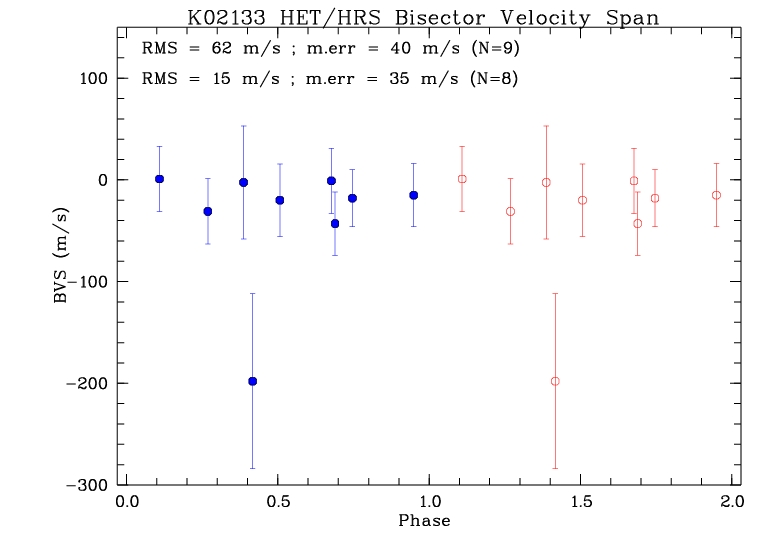
\includegraphics[width=0.50\textwidth]{k02133_bvs_phas1.jpg}
\caption{The bisector velocity spans of the nine HET observations of Kepler-91. There is a single outlier point which has a very large uncertainty. Excluding this leaves an rms scatter in the bisector velocity spans of 15 m/s. There is not obvious correlation with orbital phase.}
\label{fig:bisectors}
\end{figure}


\section{Simultaneous modeling of Kepler and RV data}
To provide a self-consistent model of both the light curve and the radial velocity observations we chose to model both datasets simultaneously using the orbital model described in \citet{rowe14}.

Significant planet-induced variability outside of the transit of Kepler-91b has been noted in previous work \citep{lillo14,esteves13}. We chose to model these light curve variations rather than remove them via filtering.  We include 5 physical components in our model of the light curve: a transit, an occultation, ellipsoidal modulation, Doppler boosting and reflection from the planet. We additionally include the radial velocity data as an additional component in the model and finally we include a model for the correlated noise.

\subsection{Parameterization}
We used a limb darkened transit model \citep{mandel02} following a quadratic limb darkening law, and a uniform disk model for the occultation. The ellipsoidal variations, Doppler boosting and reflection off the planet were modeled in the manner described by \citet{lillo14}, but we parameterized the Doppler beaming in terms of $K$, the radial velocity semi-amplitude, to retain a consistent solution between the light curve data and the spectroscopic radial velocities. The scaling between the radial velocity semi-amplitude and the Doppler beaming amplitude is proportional to a `beaming factor' $B$ such that
\begin{equation}
A_b = B \frac{K}{c} (e\cos{\omega})
\end{equation}
where $A_b$ is the semi-amplitude of the Doppler beaming signal $c$ is the speed of light and $e$ is the eccentricity and $\omega$ is the argument of periastron. We calculated $B$ in the manner described by \citet{bloemen11} to find a value of 5.46 which we kept fixed.

We parameterized the combined model in terms of $\rho$ the mean stellar density, $zp$ a photometric zero point nuisance parameter, linear ($\gamma_1$) and quadratic ($\gamma_2$) limb darkening coefficients, $T_0$ the mid-point of transit, $P$ the orbital period of the planet, $b$ the impact parameter, $R_{p}/R_{\star}$ the planet-to-star radius ratio, eccentricity vectors $e\cos{\omega}$ and $e\sin{\omega}$ where $e$ is eccentricity and $\omega$ is the argument of periastron, the amplitude of the ellipsoid variations $A_e$, the amplitude of the refection from the planet $A_r$, the occultation depth $F_e$, radial velocity semi-amplitude $K$, and $V$ a radial velocity zero-point.

Because we are using disparate data sets is it useful to include a parameter for both the light curve and radial velocity data that is an additional noise term which is added in quadrature with the formal uncertainty ($\sigma_{lc}$ and $\sigma_{rv}$). These account for missing physics on our model in addition to dealing with underestimation of the reported uncertainties. This creates a flexible model that enables us to scale the two data sets appropriately.

%\textbf{Maybe here for the section on the GP noise model. This needs to be given prominence in this paper because it's novel.}
\subsection{Gaussian Process noise model}
After examining the PDC data we noted the presence of a broad low frequency noise component in the time series. Red giants are known to show granulation (cite) to which we attribute the low frequency noise component. Not accounting for this correlated noise component can bias the observed planet parameters \citep{carter09}. \citet{huber13b} have shown this type of noise is \emph{can} be modeled by a two component (pink) noise model: a white Gaussian noise and a red noise component.

A Gaussian process is a general framework for modeling correlated noise
\citep{rasmussen} and it has been applied to transmission spectroscopy
\citep{gibson-gp,evans-gp} and Kepler light curves \citep[][Dawson
\emph{et al.}\ in press]{ambikasaran14}.
The basic idea is to model the light curve as being drawn from a large
$N_\mathrm{data}$-dimensional Gaussian where the covariance matrix $K$ is
modeled as
\begin{eqnarray}
K_{ij} &=& \sigma_i^2\,\delta_{ij} + k(t_i,\,t_j)
\end{eqnarray}
where $\sigma_i$ is the observational uncertainty, $\delta_{ij}$ is the
Kronecker delta, and $k(t_i,\,t_j)$ is the so-called \emph{covariance kernel
function} that quantifies the correlations between data points.
There is a lot of freedom in how we choose this covariance function but here
we'll choose a very simple and commonly used model called the
squared-exponential or radial basis function kernel
\begin{eqnarray}
k(t_i,\,t_j) &=& A^2\,\exp\left(-\frac{[t_i-t_j]^2}{2\,\tau^2}\right)
\end{eqnarray}
where the covariance amplitude $A$ is measured in flux units and the length
scale $\tau$ is measured in days.
When fitting the data, we marginalize over the parameters $A$ and $\tau$ with
log-uniform priors.


%However, we opted to model the noise as three sources in the frequency domain, a flat white noise component, a half-Lorentzian centered at zero frequency, and a Gaussian at the frequency of the solar-like oscillations. At each realization of the light curve model we fit a noise model to the power spectra density of the residuals when the light curve model has been subtracted from the observed flux. There are six free parameters in the noise model; a white noise background, an amplitude and width of the half-Lorentzian and the mean, standard deviation and amplitude of a Gaussian. The noise model is built upon an adaptive Wiener filter \citep{wiener49,astroML,astroMLText}. The fit performed using a bounded limited-memory Broyden-Fletcher-Goldfarb-Shanno optimization \citep{zhu97} implemented in Scipy \citep{scipy}. We opted to use a bounded optimization to keep the mean of the Gaussian component in the region of frequency space where we have prior knowledge of solar-like oscillations. The noise model is then convolved with the power spectral density of the light curve model subtracted flux and this is then transformed back into the time domain. The log-likelihood of the realization is calculated assuming a Gaussian of residuals after the noise model is subtracted from the flux.




%We opted to model the red noise as a Wiener process and account for it in our likelihood function. At realization of the model we first subtract the light curve model and then pass the data through an adaptive Wiener filter \citep{wiener49,astroML,astroMLText}, before calculating the log likelihood. The filter is adaptive because it optimizes the width and amplitude of a Gaussian function in the frequency domain. In Figure~\ref{fig:filter} we show a typical filter shape in the frequency domain.

%\begin{figure}
%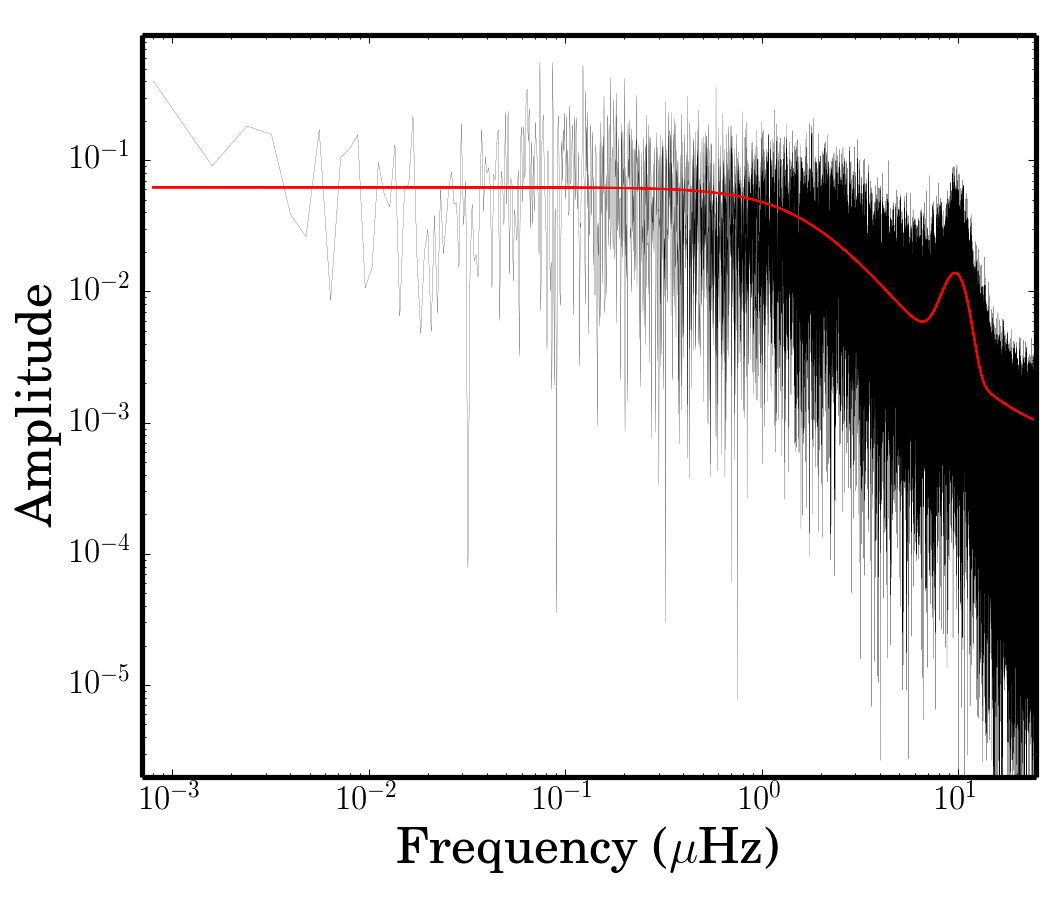
\includegraphics[width=0.50\textwidth]{filter.png}
%\caption{The power spectra density of the observe data is shown in black and a typical Wiener filter is shown in red. The filter captures the low frequency variability which we attribute to stellar granulation. }
%\label{fig:filter}
%\end{figure}

\subsection{Priors}
Priors on our model parameters are shown in Table~\ref{tab:priors}. On particular note is $\rho$ where we enforce a normal prior constrained from the probability density found from asteroseismology. We enforce a $1/e$ prior because without this our parameterization in terms of $e\sin{\omega}$ and$e\cos{\omega}$ would bias $e$ high (cite Eastman). We use a normal prior on limb darkening with the expectation obtained through interpolation of model limb darkening in the Kepler bandpass with $T_{eff}$, $\log{g}$ and [Fe/H] fixed at the values shown in Table~\ref{tab:priors}, and with a standard deviation of 0.1. Finally, we set a number of prior constraints on linear combinations of $\gamma_1$ and $\gamma_2$ that prevent them taking unphysical values \citep{burke08}.

\begin{table}
\centering
\caption{Model parameters}\label{tab:priors}
\begin{tabular}{l l }
Property & Prior \\
\hline
$\rho$		&	$N(0.0073;0.0001)$ \\
$zp$				& 	$U(-\infty;+\infty)$\\
$\gamma_1$		&	$N(0.67;0.6)$ \\
$\gamma_2$		&	$N(0.09;0.6)$\\
$T_0$ & $U(-\infty;+\infty)$\\
$P$ & $U(-\infty;+\infty)$\\
$b$ & $U(0;1+R_{p}/R_{\star})$\\
$R_{p}/R_{\star}$ & $U(0;1)$ \\
$e\cos{\omega}$ &$U(-1;1)$ \\
$e\cos{\omega}$ & $U(-1;1)$\\
$A_e$ &$U(-\infty;+\infty)$ \\
$A_r$ & $U(-\infty;+\infty)$\\
$F_e$ & $U(-\infty;+\infty)$\\
$V$ &$U(-\infty;+\infty)$ \\
$K$ &$U(-\infty;+\infty)$ \\
$\sigma_{lc}$ & $U(0;+\infty)$\\
$\sigma_{rv}$ &$U(0;+\infty)$ \\
$A_{GP}$ &  $U(0;+\infty)$ \\
$l_{GP}$ &  $U(0;+\infty)$ \\
\hline
\end{tabular}
\end{table}

\subsection{Markov-Chain Monte Carlo modeling}
We numerically integrated the posterior probability using an efficient affine invariant Markov-Chain Monte Carlo (MCMC) algorithm \citep{goodman10,foreman13}.  This method utilizes many walkers to reduce autocorrelation time; we opted to use 700 walkers each taking 15,000 steps for a total of $10.5\times10^6$ samples of the posterior probability. However, we toss the first 5,000 samples in each walker as burn-in which leaves $7\times10^6$ samples use to calculate posterior distributions.

In Figure~\ref{fig:noise model} we show two transits in Kepler data, the mean noise model, light curve model and the combined light curve and noise model. The noise model does a good job of matching red noise component of the noise.

\begin{figure}
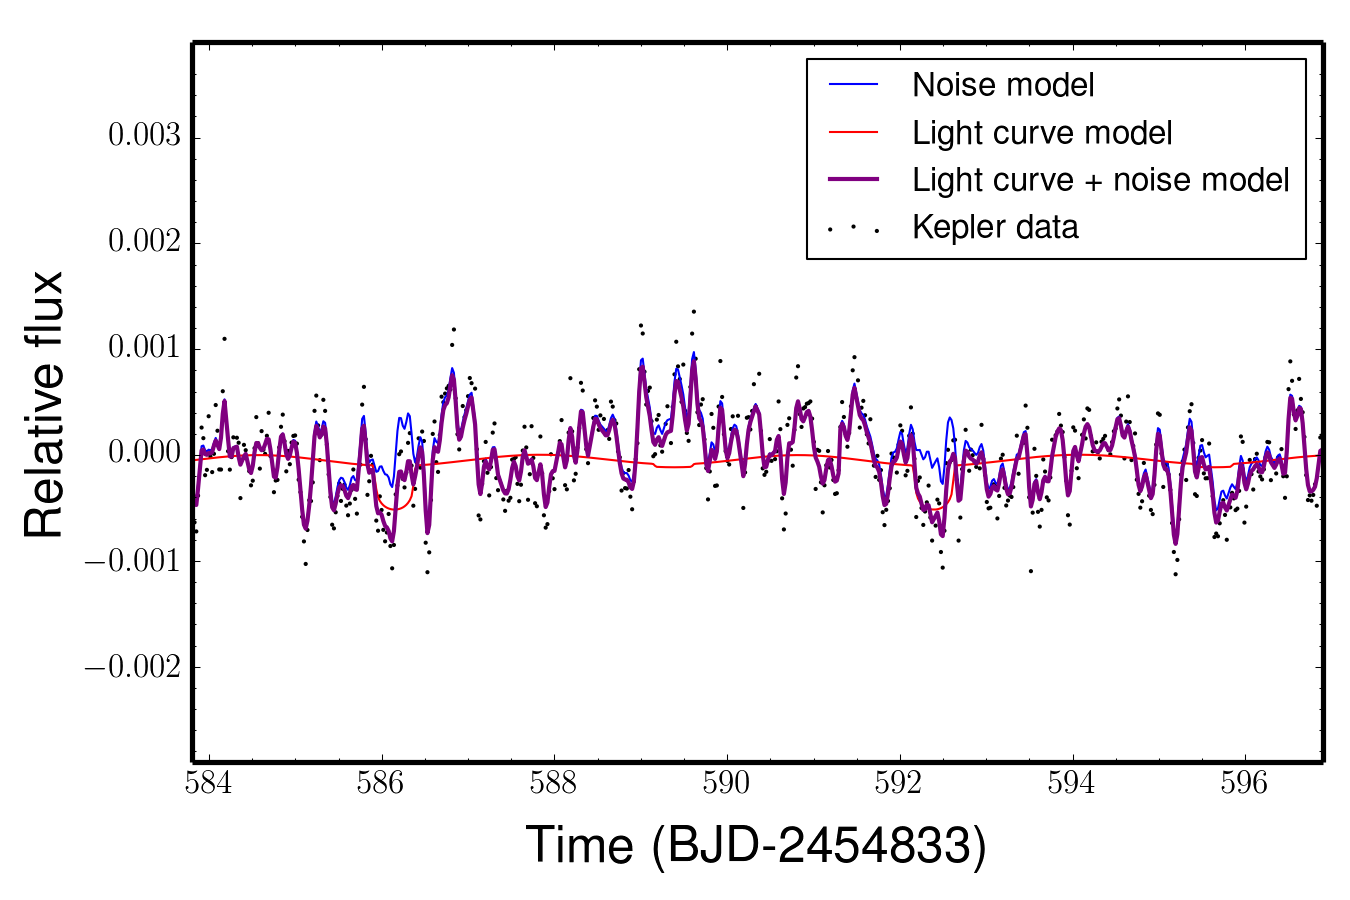
\includegraphics[width=0.50\textwidth]{noisemodel.png}
\caption{A small section of the observed Kepler data shown to demonstrate our noise model. The observed at a is shown as black points, the noise model in blue, the light curve model in red and the combined light curve and noise model in purple. Two transit are shown in plot. }
\label{fig:filter}
\end{figure}


\section{Results}
We were able to produce a self consistent model that well described the data. Parameters from the modeling are reported in Table~\ref{tab:results}, we give the median and central 68\% bounds of the marginalized posterior distribution for each parameter. In addition we state the most probably model we sampled which provides a self consistent set of parameters. Our parameter estimates are largely consistent with \citet{lillo14}. While we obtain a slightly lower estimate for $R_{p}/R_{\star}$, we are still consistent with \citet{lillo14} at the level of $<$1.5$\sigma$. Our estimate of $R_{p}/R_{\star}$ is inconsistent with that found by \citet{sliski14}.

We derive a planet mass of $0.73\pm 13$ M$_{Jup}$ which, combined with a planet radius of $1.308^{+0.061}_{-0.074}$ $R_{Jup}$ yields a density of $0.40{+0.10}_{-0.09}$ g cm$^{3}$ implying that Kepler-91b is somewhat inflated. Specifically, we highlight the consistency between the planet mass we obtain with radial velocity observations and the mass\citet{lillo14} obtains from the phase curve alone. Kepler-91b is one of a growing number of examples showing that hot Jupiter densities can be estimated from Kepler data alone \citep{welsh10,barclay12,quintana13}.

\citet{lillo14} suggest that Kepler-91b may be on an eccentric orbit. In Figure~\ref{fig:ecc} we show our posterior distribution for eccentricity derived from our $e\sin{\omega}$ and $e\cos{\omega}$ samples. While the data prefers an eccentric model, a circular orbit is not formally ruled out.

\begin{figure}
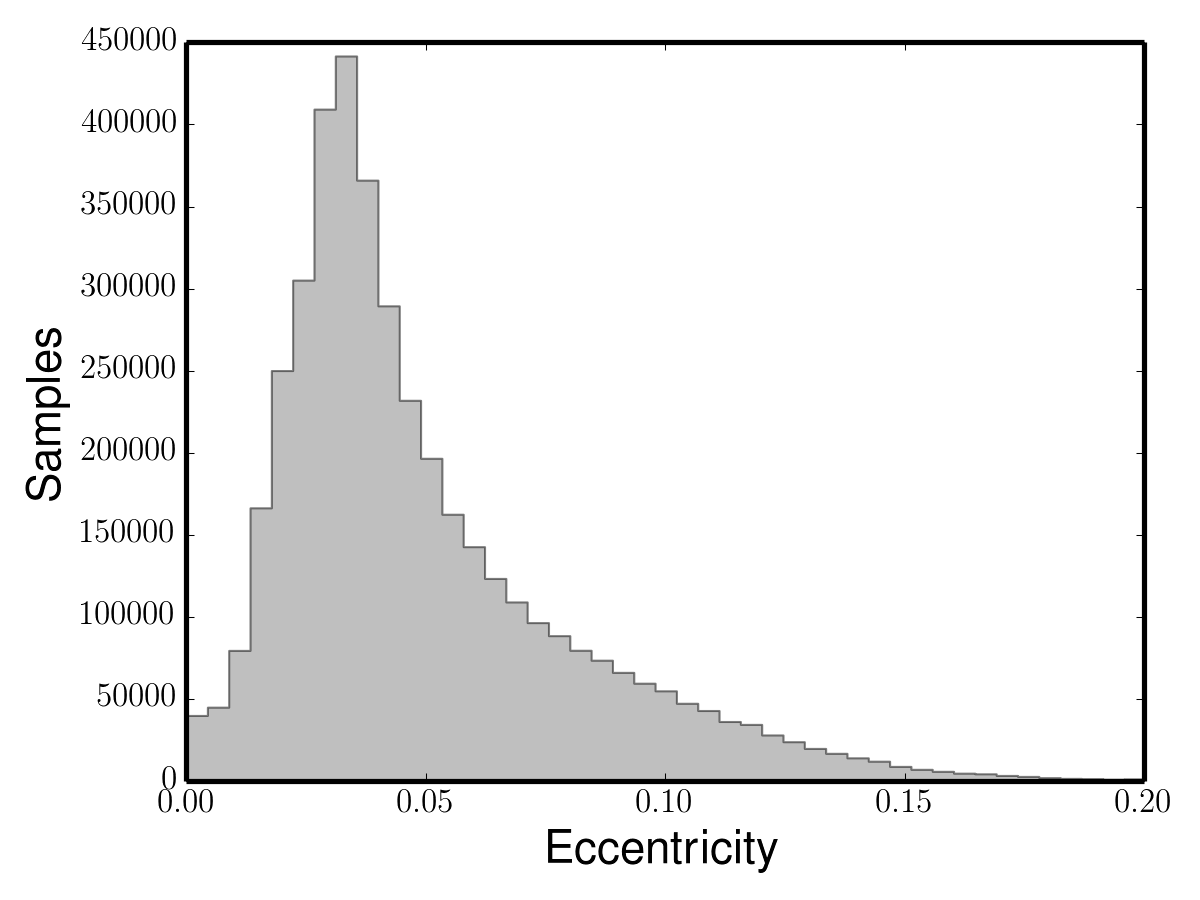
\includegraphics[width=0.50\textwidth]{ecc_hist.png}
\caption{The posterior distribution for orbital eccentricity for Kepler-91b. While a slightly eccentric orbit is preferred by the data, we cannot rule out a circular orbit model.}
\label{fig:results}
\end{figure}



\begin{figure}
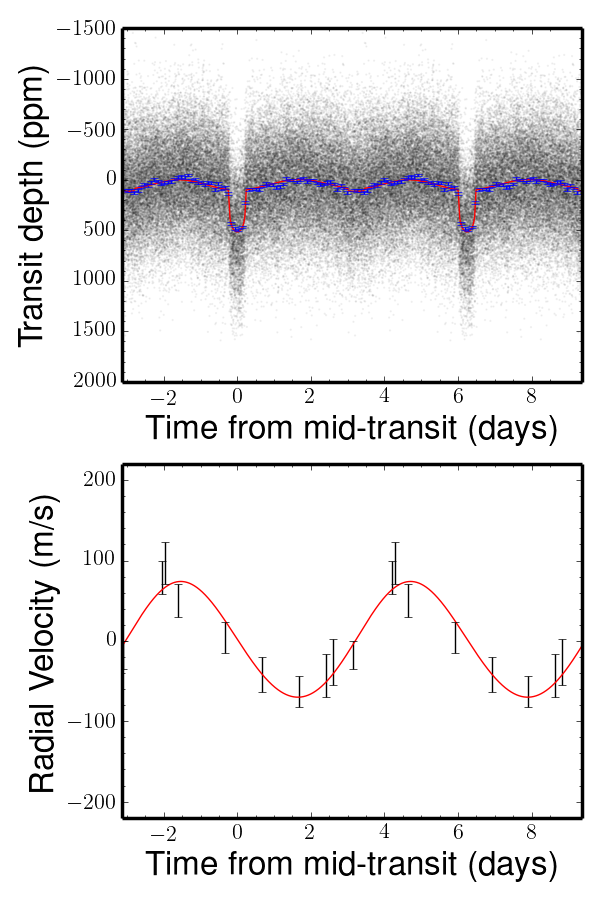
\includegraphics[width=0.50\textwidth]{koi2133.png}
\caption{The upper panel shows the observed data as black semi-transparent points. The blue points show are binned observed data with 1000 observed points included per bin. The red curve is the best fitting light curve model, excluding the noise model. The data have been folded on the orbital period of the planet and repeated twice to fully show the entire phase curve. The fit to the data does not appear especially good. However, in this figure we have not included the Gaussian Process noise model. The large scatter is owning to correlated noise in the observe data. The lower panel shows our observed radial velocity data in blue and the best fitting model in red.}
\label{fig:results}
\end{figure}

\begin{figure}
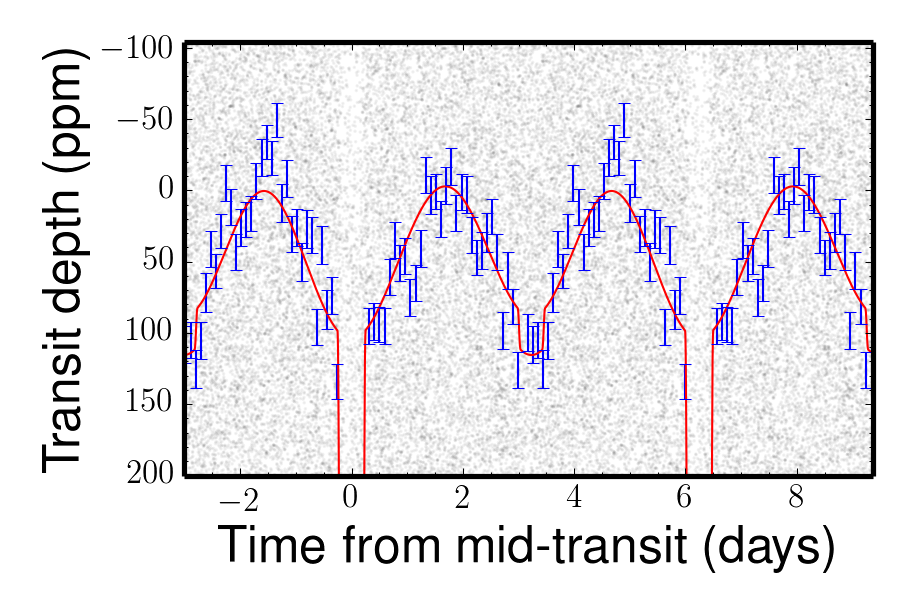
\includegraphics[width=0.50\textwidth]{koi2133_zoom.png}
\caption{This plot shows the phase variations from Kepler-91b. Is it the same data as shown in the upper panel of Figure~\ref{fig:results} but only showing the phase variations and the occultation. Similarly to in Figure~\ref{fig:results}, the correlated noise in the data implies a misleadingly poor fit of the model to the data.}
\label{fig:results_zoom}
\end{figure}

\begin{table}
\caption{Summary of posterior probabilities from the MCMC modeling. Parameters below the line break are derived from the parameters sampled by the model}\label{tab:results}
\begin{tabular}{l l l l l}
Parameter&Best fit& Median&84.1\%&15.9\%\\
\hline
%$\rho$ (g/cc)		&0.00730	& 0.00730&{+0.00010}&$-$0.00010\\
%$zp$			&-0.000057	& $-$0.000053&{+0.0000053}&$-$0.0000057\\
%$\gamma_1$	&0.18	& 0.50&{+0.48}&$-$0.35\\
%$\gamma_2$	&0.56	& 0.19&{+0.37}&$-$0.49\\
%$T_0$ (BJD-2454833)		&	136.3846& 136.3824&{+0.0043}&$-$0.0042 \\
%$P$ 	(days)		&6.246733& 6.246716&{+0.000034}&$-$0.000034\\
%$b$ 			&	0.856& 0.863&{+0.011}&$-$0.015\\
%$R_{p}/R_{\star}$& 	0.0211& 0.0213&{+0.0011}&$-$0.0008 \\
%$e\cos{\omega}$ &	0.0271& 0.0235&{+0.0086}&$-$0.0086\\
%$e\sin{\omega}$ &	$-$0.015& 0.018&{+0.054}&$-$0.030\\
%$A_e$ (ppm)		&	50.1& 51.4&{+4.8}&$-$4.9\\
%$A_r$ (ppm)		&	15& 18&{+11}&$-$10\\
%$F_e$ (ppm)		&	27& 36&{+13}&$-$13\\
%$V$ 	(m/s)		&	17.2& 16.5&{+8.2}&$-$8.0\\
%$K$ 	(m/s)		&72	& 67&{+10}&$-$10 \\
%$\sigma_{lc}$ (ppm)	&0.6	& 1.3&{+1.4}&$-$0.9  \\
%$\sigma_{rv}$ (m/s)	&	8.9& 9.0&{+8.2}&$-$6.2\\
%$A_{GP}$ (ppm)&300& 301 & {+20}&$-$20 \\
%$l_{GP}$  (days$^{2}$)&0.03729& 0.03711&{+0.00031}&$-$0.00030 \\
%
$\rho$ (g/cc)			&	0.00724		&	0.00730		&	+0.00010		&	$-$0.00010	\\
$zp$	(ppm)			&	$-$56.8		&	$-$57.5		&	+7.4			&	$-$8.8		\\
$\gamma_1$			&	0.43			&	0.50			&	+0.48		&	$-$0.35		\\
$\gamma_2$			&	0.27			&	0.19			&	+0.37		&	$-$0.49		\\
$T_0$ (BKJD\footnote{BKJD is the time system used by Kepler and is defined by Barycentric Julian Date (BJD) $-$ 2454833}) 	&	136.3837		&	136.3824		&	+0.0043		&	$-$0.0042		\\
$P$ 	(days)			&	6.246696		&	6.246716		&	+0.000034	&	$-$0.000034	\\
$b$ 					&	0.865		&	0.863		&	+0.011		&	$-$0.015		\\
$R_{p}/R_{\star}$		&	0.0212		&	0.0213		&	+0.0011		&	$-$0.0008		\\
$e\cos{\omega}$ 		&	0.0134		&	0.0234		&	+0.0086		&	$-$0.0086		\\
$e\sin{\omega}$ 		&	0.0118		&	0.0176		&	+0.054		&	$-$0.036		\\
$A_e$ (ppm)			&	50.8			&	51.5			&	+4.8			&	$-$5.0		\\
$A_r$ (ppm)			&	27.4			&	29			&	+21			&	$-$16		\\
$F_e$ (ppm)			&	49			&	39			&	+15			&	$-$15		\\
$V$ 	(m/s)				&	15.6			&	16.5			&	+8.2			&	$-$8.0		\\
$K$ 	(m/s)				&	70			&	67			&	+11			&	$-$11		\\
$\sigma_{lc}$ (ppm)		&	0.6			&	1.3			&	+1.4			&	$-$0.9		\\
$\sigma_{rv}$ (m/s)		&	8.3			&	11			&	+12			&	$-$8			\\
$A_{GP}$ (ppm)		&	301.6		&	301.2		&	+2.0			&	$-$2.0		\\
$l_{GP}$  (days$^{2}$)	&	0.03717		&	0.03711		&	+0.00031		&	$-$0.00030	\\
%
%
\hline
%$R_{p}$ ($R_{Jup}$) & 1.294 & 1.328 & +0.076 & $-$0.062 \\
%$M_{p}$ ($M_{Jup}$) & 0.78 & 0.72 & +0.12 & $-$0.11 \\
%$a/R_{\star}$ &2.469 & 2.469 & +0.011 & $-$0.011 \\
%$A_g$ & 0.37 & 0.46 & +0.18 & $-$0.17 \\
%$e$ & 0.0311 & 0.032 & +0.021 & $-$0.013 \\
%$i$ (deg)& 70.02 &  69.95 & +0.39 & $-$0.38 \\
%$\rho_{p}$ (g/cc) & 0.478 & 0.405 & +0.092 & $-$0.084\\
%
$R_{p}$ ($R_{Jup}$) 	&	1.300		&	1.308		&	+0.061		&	$-$0.074		\\
$M_{p}$ ($M_{Jup}$)	&	0.76			&	0.73			&	+0.13		&	$-$0.13		\\
$a/R_{\star}$			&	2.463		&	2.469		&	+0.011		&	$-$0.011		\\
$A_g$				&	0.66			&	0.52			&	+0.22		&	$-$0.20		\\
$e$					&	0.018		&	0.040		&	+0.040		&	$-$0.016		\\
$i$ (deg)				&	69.17		&	69.12		&	+0.58		&	$-$0.88		\\
$\rho_{p}$ (g/cc) 		&	0.43			&	0.40			&	+0.10		&	$-$0.09		\\
\hline
\end{tabular}
\end{table}

The

\section{Discussion}
We obtained good fits to both the radial velocity and light curve data with our model. The radial velocity observations phase well with the orbital period defined by the transit and therefore almost certainly are caused by a reflex motion of the star that the planet orbits. The transit model fits the data well with low eccentricity. If the density constraint from asterseismlogy were to be bad prior we would need a model with high eccentricity, which is not seen. The mass we derive is consistent with a planetary body. We therefore conclude Kepler-91b is unambiguously a planet.

This leads us to try to answer the question, what caused this to be classified as a false positive? We begin by considering the work of \citet{esteves13} who conclude that Kepler-91b is false positive based on a phase curve fit where they find a night-side temperature inconsistent with a body that is not self luminous. We do not draw the same conclusions. Using the same equation as Esteves et al for geometric albedo, we derived a value of $0.52^{+0.22}_{-0.20}$ compared with $2.49^{+0.55}_{-0.60}$ from \citeauthor{esteves13}. We hypothesize that the disparate parameter estimates arises from using different detrending techniques. Specifically we point to their use of a median filter which could result in the significantly smaller transit depth than we measure. The method we use to calculate the geometric albedo (and we presume \citeauthor{esteves13} use also) is
\begin{equation}
A_g = F_e \left(\frac{a}{R_p}\right)^{2} = F_e \left(\frac{a}{R_{\star}}\frac{R_{\star}}{R_{p}}\right)^{2} .
\end{equation}
Therefore, underestimating $R_{p}/R_{\star}$ will overestimate the albedo $A_g$. We caution that it is only because we were in possession of the radial velocity data, which raised doubts on the interpretation of \citeauthor{esteves13}, that we considered the more sophisticated noise model described here. We suggest that extreme caution should be used in deriving planet parameters where the host star is noisy on timescales comparable to the transit duration.

\citet{sliski14} only include data less than three transit durations from a transit and fit a standard transit model ignoring the out-of-transit ellipsoidal variations. They find that the mean stellar density derived purely from a transit model is not consistent with the asteroseismic density of the star. We suspect that \citeauthor{sliski14} find a higher stellar density because they neglected to include phase variations, particularly the high amplitude ellipsoidal variations found by \citet{lillo14}. The density parameter is sensitive to the duration of the transit, we hypothesize that not including out-of-transit variations caused an underestimate of the transit duration. This theory is strengthened because they report a significantly smaller planet-to-star radius ratio than we find. We caution against using just a short amount of data on either side of the transit as correctly estimating the out-of-transit flux level is essential to estimating the planet properties.



\section{Conclusions}
We combined Kepler data presented in previous studies of Kepler-91 with radial velocity data obtained from the Hobby-Eberly Telescope. We find that these data can be fit in a self consistent manner and the results lead us to conclude that Kepler-91b is a planet, validating the work of \citet{lillo14}. We hypothesize that recent work claiming this as a false positive erred owing to the challenge of modeling a star with a strong correlated noise component and relatively high amplitude out-of-transit variations. We use a Gaussian Process to model the correlated noise precent in the light curve of this red giant star. Our choice of the squared exponential kernel...

lets say how clever we are for using a GP...

All of the code used in this project is available from
{https://github.com/mrtommyb/GP\_model\_Kepler\_data} under the MIT
open-source software license.
This code (plus some dependencies) can be run to re-generate all of the
figures and results in this paper; this version of the paper was generated
with git commit \texttt{\githash} (\gitdate).

\acknowledgments
This paper includes data collected by the Kepler mission. Funding for the Kepler mission is provided by the NASA Science Mission Directorate. Some Kepler data presented in this paper were obtained from the Mikulski Archive for Space Telescopes (MAST) at the Space Telescope Science Institute (STScI). STScI is operated by the Association of Universities for Research in Astronomy, Inc., under NASA contract NAS5-26555. Support for MAST for non-HST data is provided by the NASA Office of Space Science via grant NNX09AF08G and by other grants and contracts. Our MCMC simulations were performed on the Pleiades supercomputer of the NASA Advanced Supercomputing Division at NASA's Ames Research Center. We used data obtained from The Hobby-Eberly Telescope (HET), a joint project of the University of Texas at Austin, the Pennsylvania State University, Stanford University, Ludwig-Maximilians-Universit\"{a}t M\"{u}nchen, and Georg-August-Universit\"{a}t G\"{o}ttingen. The HET is named in honor of its principal benefactors, William P. Hobby and Robert E. Eberly. We thank Ruth Angus for valuable discussions on noise sources in RV observations. E.V.Q. is supported by a NASA Senior Fellowship at the Ames Research Center, administered by Oak Ridge Associated Universities through a contract with NASA. D.H. acknowledges support by the Kepler Participating Scientist Program.



\bibliography{biblio}

\bibliographystyle{apj}


\end{document}
